\chapter{Résultats et futur}

\section{Résultats}

La figure \ref{fig:rmf_800} est un example de résultat obtenue à partir d'un bruit \textit{RIDGED MULTI FRACTAL}. 

\begin{figure}
    \centering
    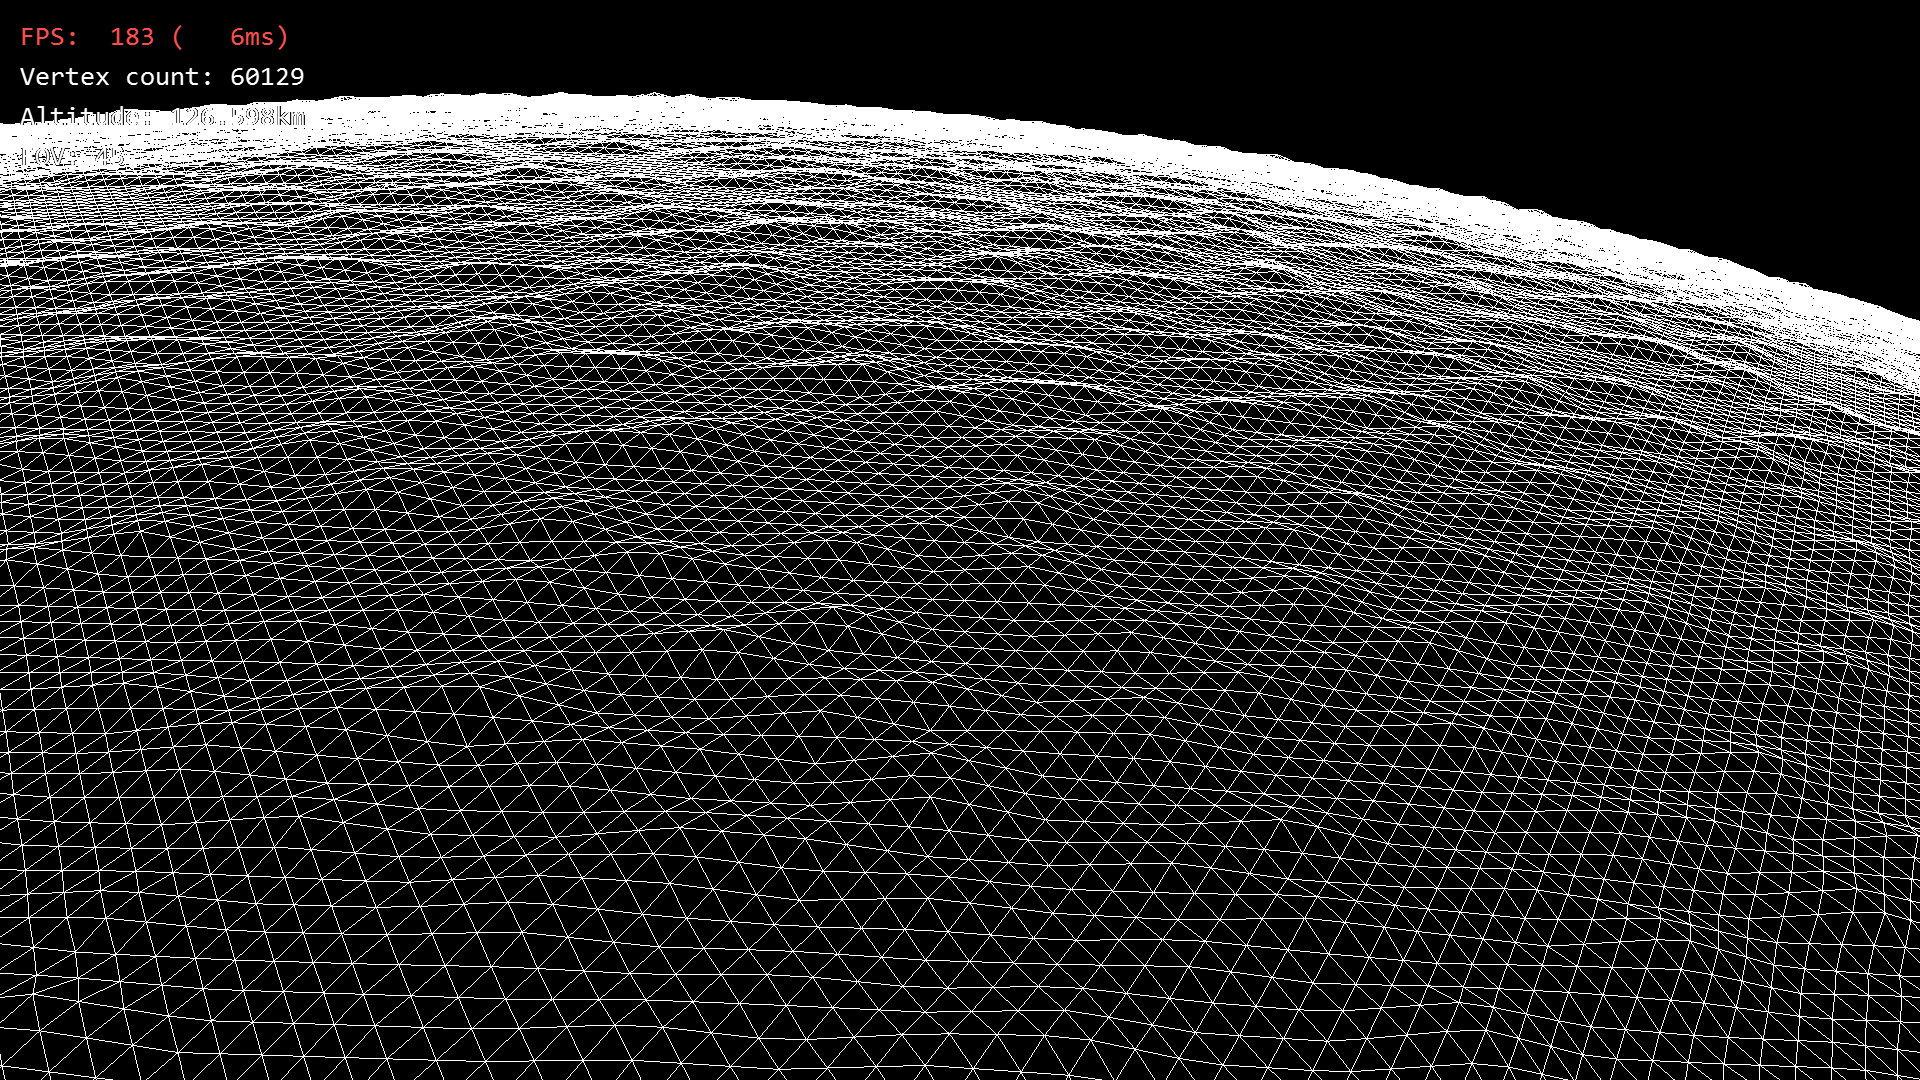
\includegraphics[width=8cm]{img/RMFV_w800_h800_wire_0.png}
    \caption{./ProceduralPlanet RIDGED-MULTI-FRACTAL --width=800 --height=800}
    \label{fig:rmf_800}
\end{figure}

Ce bruit est un bruit basé sur simplex, la figure \ref{fig:rmf} est une représentation sur deux dimension de ce bruit. 
Le bruit de la figure \ref{fig:rmf} et le bruit appliqué sur la planète ne sont pas identique, la figure \ref{fig:rmf} n'est qu'une représentation.

\begin{figure}
    \centering
    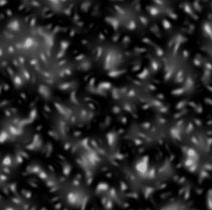
\includegraphics[width=8cm]{img/RMF.jpg}
    \caption{RIDGED MULTI FRACTAL, source \url{https://github.com/simongeilfus/SimplexNoise}, dernier accès Mars 2018}
    \label{fig:rmf}
\end{figure}



\subsection{Limitation}

Pour avoir une planète correcte, on peut voir qu'il est nécessaire de créer une carte de hauteur de faible résolution. Cependant cela fait apparaître de la pixelisation sur la planète. Cela est du au calcul de la lumière faite dans le \textit{shader} qui ce base sur les hauteurs.

\section{Futur}

